\documentclass[11pt]{article}

% ── Core packages ──────────────────────────────────────────────
\usepackage[margin=1in]{geometry}
\usepackage{amsmath,amssymb,amsthm}
\usepackage{graphicx}
\usepackage{booktabs}
\usepackage{array}
\usepackage{hyperref}
\usepackage{xcolor}
\usepackage{algorithm}
\usepackage{algpseudocode}
\usepackage{tikz}
\usepackage{pgfplots}
\pgfplotsset{compat=1.18}
\usetikzlibrary{arrows.meta, positioning, shapes.geometric, fit, backgrounds}

% ── Theorem environments ────────────────────────────────────────
\newtheorem{theorem}{Theorem}
\newtheorem{definition}{Definition}
\newtheorem{invariant}{Invariant}

% ── Hyperlink colours ───────────────────────────────────────────
\hypersetup{
  colorlinks=true,
  linkcolor=blue!60!black,
  citecolor=blue!60!black,
  urlcolor=blue!60!black
}

% ── Title ───────────────────────────────────────────────────────
\title{\textbf{Resonance is All You Need: A Dissipative Dynamical\\
System for Associative Memory in Large Language Models}}

\author{Affan Tanke\\
\small Independent Researcher, Pune, India\\
\small \href{https://github.com/your-repo-here}{github.com/your-repo-here}
}

\date{}

% ════════════════════════════════════════════════════════════════
\begin{document}
\maketitle

% ── Abstract ────────────────────────────────────────────────────
\begin{abstract}
Large language models demonstrate remarkable reasoning capabilities but
suffer from two critical limitations: lack of persistent memory and
collapse at logical phase transitions. Current retrieval-augmented
generation approaches treat memory as a semantic database, relying on
vector similarity to surface relevant information. This paradigm fails
catastrophically when causal chains span semantic discontinuities or
when logical complexity exceeds the model's intrinsic reasoning
threshold. We introduce \textbf{Resonance Memory Mesh (RMM)}, an
architecture that models memory as a dissipative dynamical system where
retrieval emerges from energy propagation through topological structure.
By offloading causal chain traversal to an external substrate, RMM acts
as a cognitive stabilizer that maintains retrieval coherence across
semantic discontinuities where standard semantic search collapses. We
demonstrate that associative recall, modeled as a physical process
rather than a spatial search problem, enables retrieval across a
five-hop causal chain where traditional methods achieve infinite rank ---
while maintaining 0.36\,ms query latency through a zero-copy Rust
kernel.
\end{abstract}

% ── 1. Introduction ─────────────────────────────────────────────
\section{Introduction}

The transformer architecture revolutionized natural language processing
by showing that attention mechanisms could replace recurrence for
sequence modeling~\cite{vaswani2017attention}. However, transformers
remain stateless---each inference operates in isolation, disconnected
from accumulated context. More critically, recent work by Zhang et
al.~\cite{zhang2026lpt} has identified a fundamental limit in large
language model reasoning: the \textbf{Logical Phase Transition (LPT)}.
They demonstrate that model accuracy does not degrade smoothly with
complexity; instead, it collapses abruptly beyond a critical
threshold---effectively a ``melting point'' for logic.

The standard solution, retrieval-augmented generation
(RAG)~\cite{lewis2020rag}, augments model inputs with relevant memories
retrieved through semantic search. However, this approach embodies what
we term the \textbf{Flashcard Fallacy}: the assumption that memory can
be adequately modeled as independent facts indexed by vector similarity.
While cosine distance in embedding space correlates with semantic
relatedness, it fails as a proxy for inferential relevance when causal
chains span semantic discontinuities. As the Logical Complexity Metric
(LoCM) increases, internal attention mechanisms fail to maintain
long-range causal coherence, triggering the phase transition collapse.

We propose reconceptualizing memory retrieval as a physical process that
operates external to the model's internal reasoning. Rather than
searching for semantic matches, we model memory as an energy-based
dynamical system~\cite{hopfield1982} where query activation initiates
energy propagation through weighted edges. Relevant memories surface
through resonance---the natural tendency of coupled systems to activate
in response to perturbation---independent of semantic similarity. By
offloading causal chain traversal to a deterministic topological
substrate, RMM acts as a cognitive stabilizer that maintains reasoning
coherence across complexity thresholds where internal attention
mechanisms fail.

To be clear, we are not suggesting RMM replaces attention.
\textit{Attention is for processing; the mesh is for retention.}

\paragraph{Contributions.}
\begin{itemize}
  \item A mathematical framework treating memory as a dissipative system
        with provable stability guarantees.
  \item Empirical validation demonstrating retrieval across a multi-hop
        semantic discontinuity where traditional methods fail.
  \item A bimodal architecture achieving sub-millisecond query latency
        through hardware-software co-design.
  \item Operational mechanisms (competitive inhibition, value-based
        eviction) enabling production deployment.
\end{itemize}

% ── 2. Related Work ─────────────────────────────────────────────
\section{Related Work}

\paragraph{Associative Memory Systems.}
Hopfield networks~\cite{hopfield1982} introduced energy-based models for
associative recall, demonstrating that memory could emerge from
minimizing energy functionals. Kohonen's self-organizing
maps~\cite{kohonen1972} showed how topological structure could capture
semantic relationships. Our work extends these foundations to
graph-structured memory with controlled dissipation dynamics.

\paragraph{Spreading Activation.}
Collins and Loftus~\cite{collins1975} proposed spreading activation as a
model of human semantic memory, where concepts activate related concepts
through weighted connections. Anderson~\cite{anderson1983} formalized
this as a computational model. RMM implements spreading activation with
explicit stability guarantees and engineering optimizations for
production deployment. Crucially, classical spreading activation models
lack convergence guarantees and were never designed for production
deployment at scale; RMM adds provable stability via Theorem~\ref{thm:convergence}
and a Rust execution kernel that enforces bounded latency.

\paragraph{Memory-Augmented Neural Networks and Graph Retrieval.}
Weston et al.~\cite{weston2015} introduced memory networks for reading
and writing to external memory. Lewis et al.~\cite{lewis2020rag}
demonstrated standard RAG for knowledge-intensive tasks. RAPTOR~\cite{sarthi2024raptor}
extends RAG through recursive tree-based abstractive summarization,
improving multi-hop coverage but still relying on embedding-space
retrieval as the primary entry mechanism. HippoRAG~\cite{gutierrez2024hipporag},
drawing inspiration from hippocampal indexing theory, uses a knowledge
graph to connect related passages; however, it still depends on semantic
similarity for graph entry, leaving the semantic discontinuity problem
unsolved. Recent systems like GraphRAG and Graphiti similarly remain
static knowledge repositories that fail when the entry vector cannot
locate the correct starting node. A concurrent taxonomy of agent memory
systems~\cite{hu2025memory} organizes memory by form, function, and
dynamics; our contribution specifically addresses the retrieval dynamics
dimension, demonstrating that topology-driven propagation outperforms
embedding-space search for causally structured knowledge.

\paragraph{Logical Reasoning Limits.}
Zhang et al.~\cite{zhang2026lpt} recently identified Logical Phase
Transitions in LLM reasoning---critical complexity thresholds beyond
which model accuracy collapses abruptly to near-random performance. They
propose neuro-symbolic curriculum tuning to delay this transition from
within the model. We take a different approach: rather than fighting the
phase transition from inside the model's architecture, we offload the
topological load to an external memory substrate. By maintaining causal
chains in an external dissipative system, RMM circumvents the transition
entirely.

\paragraph{Energy-Based and Modern Hopfield Associative Memory.}
Ramsauer et al.~\cite{ramsauer2020hopfield} showed that modern
continuous Hopfield networks with polynomial energy functions have
exponentially large storage capacity, formalizing the theoretical basis
for high-dimensional associative recall. Kanerva's Sparse Distributed
Memory~\cite{kanerva1988} similarly demonstrated that distributed
content-addressable memory can retrieve information under partial or
noisy cues. RMM inherits this associative philosophy but externalizes it
as a graph substrate with explicit causal topology rather than as a
weight matrix.

\paragraph{Vector Search Infrastructure.}
Modern vector databases use approximate nearest neighbor
algorithms~\cite{johnson2019} with HNSW indices~\cite{malkov2018} for
efficient similarity search. These provide entry-point identification
for RMM but cannot replace resonance-based propagation for causal
retrieval.

% ── 3. The Flashcard Fallacy ────────────────────────────────────
\section{The Flashcard Fallacy}

Traditional RAG operates through a straightforward pipeline: embed the
query, retrieve top-$K$ semantically similar documents, inject context
into the LLM prompt. This has computational complexity
$\mathcal{O}(d \cdot \log N)$ for approximate nearest neighbour search
where $d$ is embedding dimension and $N$ is corpus size.

The fundamental limitation lies not in computational characteristics but
in the semantic similarity assumption. A memory may be critically
relevant through chains of logical implication while sharing minimal
vocabulary with the query.

\begin{definition}[Semantic Discontinuity]
Let $A$ and $E$ be memory nodes connected by a causal chain
$A \to B \to C \to D \to E$. We say there exists a
\emph{semantic discontinuity} if
$\cos(\mathbf{v}_A, \mathbf{v}_E) < \tau$,
where $\mathbf{v}_A, \mathbf{v}_E$ are embedding vectors and $\tau$ is
the retrieval threshold (typically $0.3$--$0.5$).
\end{definition}

When semantic discontinuities occur, RAG fails regardless of retrieval
depth $K$ because the target node never enters the candidate set. This
represents a categorical limitation---the system cannot retrieve what it
cannot find through similarity search.

% ── 4. Resonance Memory Mesh ────────────────────────────────────
\section{Resonance Memory Mesh}

We treat memory not as a database but as a physical system governed by
energy dynamics. Each node possesses an energy state that responds to
incoming activation. Energy propagates through weighted edges according
to dissipative dynamics, gradually decaying while spreading through the
mesh.

\begin{definition}[Resonance]
We use the term \emph{resonance} to describe the phenomenon where a node
accumulates energy from multiple upstream sources within a single
propagation step. In the BFS propagation kernel, energy transfers from
all active frontier nodes are summed per-target before activation
(Algorithm~\ref{alg:bfs}, step~2c). A node \emph{resonates} when its
topological position causes it to receive energy from multiple
convergent paths simultaneously, resulting in accumulated activation
exceeding that of any single incoming path. This mechanism is analogous
to constructive interference in coupled physical systems and
distinguishes RMM from single-path graph traversal.
\end{definition}

\subsection{Node Initialization and Initial Energy Assignment}

Before resonance propagation begins, seed nodes must be identified and
injected with an initial energy payload in three steps.

\textbf{Step~1 --- Seed Identification.}
Given a query vector $\mathbf{q} \in \mathbb{R}^d$, the system computes
cosine similarity against all node embeddings in the L2 store:
\begin{equation}
  \operatorname{sim}(\mathbf{q}, \mathbf{v}_i)
  = \frac{\mathbf{q} \cdot \mathbf{v}_i}{\|\mathbf{q}\|\,\|\mathbf{v}_i\|}
\end{equation}
Nodes exceeding similarity threshold $\tau$ (or the top-$K$ nodes) are
designated as candidate seed nodes.

\textbf{Step~2 --- Hybrid Ignition Score.}
Candidate seed nodes are ranked by a blended score combining semantic
similarity with node significance, weighted by mixing coefficient
$\alpha_{\mathrm{ign}} \in [0,1]$ (default $0.7$):
\begin{equation}
  \operatorname{score}(i)
  = \alpha_{\mathrm{ign}} \cdot \operatorname{sim}(\mathbf{q}, \mathbf{v}_i)
  + (1 - \alpha_{\mathrm{ign}}) \cdot S(i)
\end{equation}
The top-$K_{\mathrm{seed}}$ candidates become the active seed set
$\mathcal{S}$.

\textbf{Step~3 --- Energy Injection.}
Each seed node $i \in \mathcal{S}$ receives a fixed initial energy
payload scaled by its significance:
\begin{equation}
  e_i(0) = E_{\max} \cdot S(i), \qquad
  e_j(0) = 0 \text{ for } j \notin \mathcal{S}
\end{equation}

This initialization is the \emph{only} point at which semantic
similarity influences RMM's retrieval process. All subsequent reasoning
occurs through topological propagation, entirely independent of
embedding space geometry.

\subsection{Mathematical Formulation}

Let $G = (V, E, W)$ be a directed weighted memory graph where $V$
contains memory nodes, $E$ contains edges, and
$W: E \to \mathbb{R}^+$ assigns positive edge weights.

\textbf{State Update Rule.} The energy state evolves according to:
\begin{equation}\label{eq:update}
  e_j(t+1) = \operatorname{clip}_{[0,1]}\!\left(
    e_j(t)\,e^{-\lambda\Delta t}
    + \sum_{i \in \mathcal{F}_t} e_i(t)\,\beta\,w_{ij}
  \right)
\end{equation}
where $\lambda$ is the decay constant, $\beta \in (0,1)$ is the
dissipative gain factor, $\mathcal{F}_t \subseteq V$ is the active
frontier (nodes with $e > \varepsilon$), and $w_{ij} \in [0,1]$ is the
edge weight from node $i$ to $j$.

\textit{Note:} $S(i)$ influences initial energy injection at node $i$
(\S4.1) but does not appear in the per-hop transfer rule; this keeps the
update equation analytically clean.

\textbf{Stability Conditions.}

\begin{invariant}[Energy Dissipation]
We enforce $\beta < 1$ through parameter selection. Combined with
exponential decay and clamping to $[0,1]$, energy cannot accumulate
without external input.
\end{invariant}

\begin{invariant}[Per-Edge Weight Bound]
For all edges, $w_{ij} \in [0,1]$. Combined with $\beta < 1$, the
transfer $e_i \cdot \beta \cdot w_{ij} < e_i$, so no source node can
project more energy than it possesses.
\end{invariant}

\begin{theorem}[Convergence]\label{thm:convergence}
Under Invariants~1 and~2 and with seed injection occurring only at
$t=0$, the system converges to $e_j = 0$ for all $j$ in at most $H$
steps, where $H$ is the BFS hop limit.
\end{theorem}

\begin{proof}
Seed nodes receive energy $e_i(0) = E_{\max} \cdot S(i)$, a one-time
injection. For all subsequent hops $t \ge 1$, no external energy enters
the system. At each hop: (i)~existing energy decays by factor
$e^{-\lambda\Delta t} < 1$; (ii)~transferred energy is bounded by
$e_i(t)\,\beta\,w_{ij} < e_i(t)$ (Invariant~2, $\beta < 1$);
(iii)~the clip operation enforces $e_j \le 1$. The BFS terminates after
$H$ hops by construction, at which point no further propagation occurs.
With $\beta < 1$ and $\lambda > 0$, subsequent passive decay drives all
energies to zero.
\end{proof}

\subsection{Competitive Inhibition}

As the mesh scales, uncontrolled spreading can lead to saturation. To
prevent this ``heat death,'' we implement competitive inhibition
inspired by lateral inhibition in neural systems. When total mesh energy
exceeds threshold $E_{\max}$, all active nodes are globally normalized:
\begin{equation}
  e_i \leftarrow e_i \cdot \frac{E_{\max}}{\displaystyle\sum_{j \in \mathcal{A}} e_j}
\end{equation}
where $\mathcal{A}$ is the set of active nodes. This forces nodes to
compete for limited activation capacity, ensuring only the most resonant
causal paths survive propagation.

\subsection{Computational Complexity}

The propagation phase has complexity $\mathcal{O}(H \cdot F)$ where $H$
is the maximum number of hops and $F$ is the maximum frontier size per
hop. Since $H$ and $F$ are design-time constants ($H=5$, $F=50$ by
default), propagation is $\mathcal{O}(1)$ with respect to corpus size
$N$ after entry-point identification---a constraint-bounded constant
that trades exhaustive traversal for deterministic latency at any graph
scale. This contrasts with standard RAG's $\mathcal{O}(K)$ retrieval
phase.

Table~\ref{tab:hyperparams} lists all system hyperparameters.

\begin{table}[h]
\centering
\caption{System Hyperparameters}
\label{tab:hyperparams}
\begin{tabular}{llrl}
\toprule
\textbf{Parameter} & \textbf{Symbol} & \textbf{Default} & \textbf{Description} \\
\midrule
Dissipative gain       & $\beta$              & $0.5$   & Energy transfer fraction per hop \\
Decay rate             & $\lambda$            & $0.1$   & Exponential decay constant (per second) \\
Max hops               & $H$                  & $5$     & BFS depth limit \\
Energy ceiling         & $E_{\max}$           & $10.0$  & Competitive inhibition threshold \\
Activation threshold   & $\varepsilon$        & $0.01$  & Minimum energy to remain active \\
Max neighbours         & $F$                  & $50$    & Frontier cap per hop \\
Min edge weight        & $w_{\min}$           & $0.05$  & Edge filter floor \\
AutoLink threshold     & $\tau_{\text{link}}$ & $0.6$   & Min cosine similarity to create edge \\
Ignition blend         & $\alpha_{\text{ign}}$& $0.7$   & Similarity vs.\ significance weight (\S4.1) \\
Hub dampening          & $\alpha_{\text{hub}}$& $0.5$   & Log-scale dampening for high-degree hubs (\S5) \\
Seed candidates        & $K_{\text{seed}}$    & $3\times\text{top\_n}$ & Candidate pool for Hybrid Ignition (\S4.1) \\
\bottomrule
\end{tabular}
\end{table}

\subsection{Node Significance \texorpdfstring{$S(i)$}{S(i)}}

$S(i) \in [0,1]$ is the \textbf{Node Significance} scalar assigned at
ingestion time (default $S(i) = 1.0$). Its role is two-fold: (i)~it
scales the initial energy payload at seed nodes; (ii)~it controls
eviction priority via the V-LRU score (\S6). It does not modulate
per-hop transfer, keeping the propagation rule analytically separable
from the salience model.

The biological analogy is apt---the brain consolidates and associates
high-affect events more broadly~\cite{collins1975}. RMM implements this
by giving high-significance nodes a larger initial energy payload,
allowing resonance to spread further through their causal neighbourhood.
This mirrors significance-weighted mechanisms in Sparse Distributed
Memory~\cite{kanerva1988} and continuous Hopfield
networks~\cite{ramsauer2020hopfield}.

\subsection{RAG as a Degenerate Case}

By parameterizing retrieval physically, RMM creates a tunable
``cognition dial.'' Table~\ref{tab:modes} shows the three operational
modes.

\begin{table}[h]
\centering
\caption{RMM Operational Modes}
\label{tab:modes}
\begin{tabular}{llll}
\toprule
\textbf{Mode} & \textbf{$\beta$} & \textbf{$\lambda_{\text{decay}}$} & \textbf{Behaviour} \\
\midrule
Strict   & $< 0.3$ & high & Behaves identically to standard RAG \\
Standard & $0.7$   & $0.5$  & Associative memory \\
Creative & $> 0.85$ & low  & Expansive, multi-hop deduction \\
\bottomrule
\end{tabular}
\end{table}

When operating with low $\beta$ and high $\lambda_{\text{decay}}$, RMM
strictly reproduces standard RAG behaviour. This strongly indicates that
retrieval-augmented generation is not an alternative architecture, but
rather a degenerate special case of RMM---RAG with the reasoning turned
off.\footnote{Notably, the industry standard for ``advanced memory''
corresponds mathematically to near-zero gain, suggesting the field has
optimized extensively within a degenerate parameter regime.}

% ── 5. System Architecture ──────────────────────────────────────
\section{System Architecture}

\begin{algorithm}[t]
\caption{AtomicPing BFS Propagation}
\label{alg:bfs}
\begin{algorithmic}[1]
\Require entry\_ids $\mathcal{S}$, cache $L_1$,
         config $(\beta, \lambda, H, F, \varepsilon, E_{\max})$
\Ensure ranked node list by accumulated energy
\For{each $s \in \mathcal{S}$}
  \State $e_s \leftarrow E_{\max} \cdot S(s)$ \Comment{Ignition}
  \State frontier $\leftarrow$ frontier $\cup \{s\}$
\EndFor
\For{hop $= 1$ \textbf{to} $H$}
  \State transfers $\leftarrow \{\}$
  \For{each src $\in$ frontier \textbf{(parallel)}}
    \For{each edge $(\text{src} \to j,\, w_{ij})$ in top-$F$ neighbours of src $[w \ge w_{\min}]$}
      \State $e_{\text{transferred}} \leftarrow e_{\text{src}} \cdot \beta \cdot w_{ij} \cdot \gamma(\deg(\text{src}))$
      \If{$e_{\text{transferred}} \ge \varepsilon$}
        \State transfers$[j]$ $+= e_{\text{transferred}}$
      \EndIf
    \EndFor
  \EndFor
  \For{each target $j \in$ transfers}
    \State $e_j \leftarrow \operatorname{clip}(e_j \cdot e^{-\lambda\Delta t} + \text{transfers}[j],\; 0,\; 1)$
  \EndFor
  \State frontier $\leftarrow \{j \in \text{transfers} \mid j \text{ not yet visited as source}\}$
\EndFor
\State Apply competitive inhibition (\S4.3)
\State \Return nodes sorted by $e_j$ descending
\end{algorithmic}
\end{algorithm}

where $\gamma(d)$ is the hub-dampening factor:
$\gamma = 1.0$ if $d \le$ hub\_threshold, else
$1 / (1 + \alpha_{\text{hub}} \cdot \ln(d / \text{hub\_threshold}))$.
Note: $\alpha_{\text{hub}}$ and $\alpha_{\text{ign}}$ are distinct
parameters (Table~\ref{tab:hyperparams}). Theorem~\ref{thm:convergence}
sets $\gamma = 1.0$ for analytical simplicity; hub dampening is an
implementation-level stabilizer and does not affect the convergence
guarantee.

\subsection{Bimodal Memory Design}
\textbf{L1 Cache (Active Mesh).} Propagation-critical state resides in a
Rust kernel using lock-free concurrent data structures (DashMap)
maintaining current energy states, edge weights, and the frontier queue.

\textbf{L2 Store (Persistent Graph).} PostgreSQL with pgvector
extensions provides durable storage for graph topology, embeddings, and
metadata.

\subsection{Zero-Copy FFI Bridge}
Node identifiers are passed as raw 16-byte UUID buffers, and the pointer
to L1 memory is passed directly to Rust, eliminating serialization
during multi-hop propagation. This design achieves the measured
0.36\,ms hot query latency.

\subsection{Asynchronous Write-Back}
Energy state updates are buffered in a sharded mutex structure. A
background thread periodically flushes buffers to L2. If database writes
fail, updates are merged back into the buffer rather than discarded,
ensuring no memory loss.

\subsection{Graph Construction}
Edges are constructed automatically at ingestion time via the
\textbf{AutoLinker} module. Nodes exceeding proximity threshold
$\tau_{\text{link}}$ (default $0.6$) are connected with bidirectional
edges whose weights equal the measured cosine similarity, capped at
$K_{\text{link}} = 10$ nearest neighbours. Manual edges can be added
via the \texttt{connect()} API for causal relationships not captured by
embedding proximity.

\subsection{Predictive Batch Warming}
When a node is faulted into L1 from L2, we perform a predictive batch
fetch of its top-$K$ strongest neighbours ($K = 10$), guaranteeing
exactly two database round trips to populate an entire local
neighbourhood.

% ── 6. Value-Based Eviction ─────────────────────────────────────
\section{Value-Based Eviction}

Standard LRU policies prove inadequate for memory systems because they
fail to account for structural importance. We introduce
\textbf{Value-based Least Recently Used (V-LRU)} eviction scoring:
\begin{equation}
  \operatorname{EvictionScore}_i
  = \frac{\operatorname{Recency}_i}{\operatorname{Significance}_i}
\end{equation}
This protects topological ``bridges'' (high-significance nodes) while
evicting disconnected leaf nodes.

% ── 7. Experimental Validation ──────────────────────────────────
\section{Experimental Validation}

We designed experiments to isolate RMM's core claim: the ability to
traverse semantic discontinuities through topological reasoning.

\subsection{The Bob/Alice/Mars Capital Benchmark}

The five-hop causal chain below is constructed to induce total semantic
separation between entry and target nodes:

\begin{enumerate}
  \item \textbf{Node 1 (Query Entry):} ``Bob was recently hired as
        Managing Director at Mars Capital.''
  \item \textbf{Node 2:} ``Mars Capital led the pivotal Series~A funding
        round for Alice's startup, TechCorp.''
  \item \textbf{Node 3:} ``TechCorp's flagship product relies on
        specialized hardware from Quantum Silicon.''
  \item \textbf{Node 4:} ``Quantum Silicon was recently acquired by a
        holding company, Apex Holdings.''
  \item \textbf{Node 5 (Target):} ``Apex Holdings finalized an exclusive
        enterprise contract with Omega Inc.''
\end{enumerate}

\textbf{Query:} ``Does Bob have any connection to Omega Inc.?''

The cosine similarity between Node~1 and Node~5 is precisely
$\cos(\mathbf{v}_1, \mathbf{v}_5) = 0.28$, placing the query and target
in orthogonal regions of embedding space. RAG fails because the target
node never exceeds the minimum retrieval threshold.

All benchmark results use Standard mode parameters:
$\beta = 0.7$, $\lambda = 0.1$, $H = 5$, $F = 50$,
$\varepsilon = 0.005$ (Table~\ref{tab:modes}).

Figure~\ref{fig:energy} illustrates the energy propagation dynamics.

% ── Figure 1 ──────────────────────────────────────────────────
\begin{figure}[t]
\centering
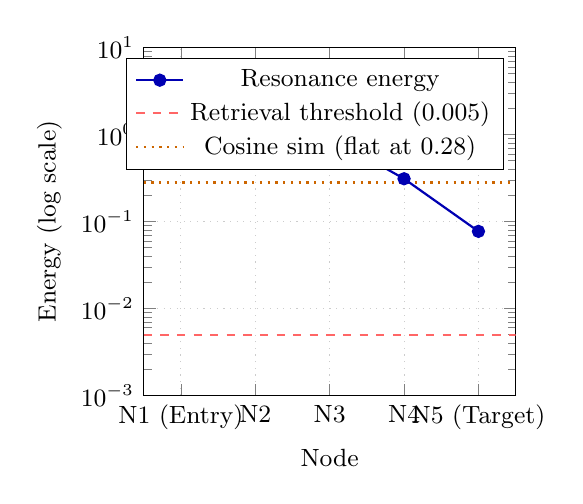
\begin{tikzpicture}
% ── Energy curve (log scale) ───────────────────────────────────
\begin{axis}[
  name=left,
  width=0.52\textwidth, height=6cm,
  xlabel={Node},
  ylabel={Energy (log scale)},
  ymode=log,
  ymin=0.001, ymax=10,
  xtick={1,2,3,4,5},
  xticklabels={N1 (Entry), N2, N3, N4, N5 (Target)},
  xmin=0.5, xmax=5.5,
  grid=major,
  grid style={dotted, gray!40},
  legend style={at={(0.97,0.97)},anchor=north east, font=\small},
  tick label style={font=\small},
  label style={font=\small},
]
\addplot[
  color=blue!70!black,
  thick,
  mark=*,
  mark options={fill=blue!70!black}
] coordinates {(1,3.09)(2,1.87)(3,0.94)(4,0.31)(5,0.077)};
\addlegendentry{Resonance energy}

\addplot[
  color=red!60,
  dashed,
  thick,
  no marks
] coordinates {(0.5,0.005)(5.5,0.005)};
\addlegendentry{Retrieval threshold (0.005)}

\addplot[
  color=orange!80!black,
  dotted,
  thick,
  no marks
] coordinates {(0.5,0.28)(5.5,0.28)};
\addlegendentry{Cosine sim (flat at 0.28)}
\end{axis}
\end{tikzpicture}

\vspace{0.5em}
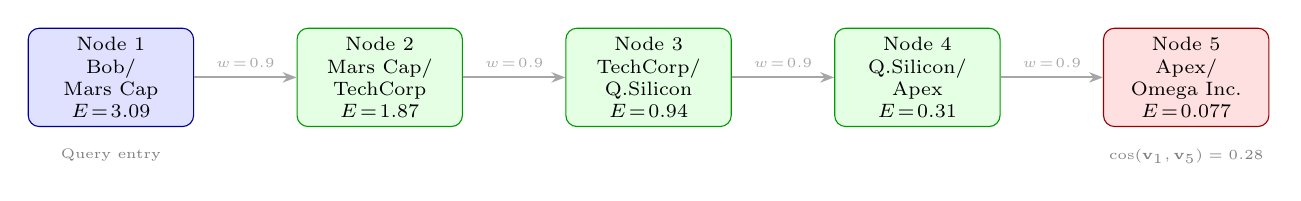
\begin{tikzpicture}[
  node distance=1.3cm,
  box/.style={
    draw, rounded corners=4pt, minimum width=2.1cm,
    minimum height=1.1cm, align=center, font=\scriptsize
  },
  entry/.style={box, fill=blue!12, draw=blue!60!black},
  mid/.style={box, fill=green!10, draw=green!60!black},
  target/.style={box, fill=red!12, draw=red!60!black},
  arr/.style={-{Stealth[length=5pt]}, gray!70, thick}
]
\node[entry]  (n1) {Node 1\\Bob/\\Mars Cap\\$E\!=\!3.09$};
\node[mid, right=of n1] (n2) {Node 2\\Mars Cap/\\TechCorp\\$E\!=\!1.87$};
\node[mid, right=of n2] (n3) {Node 3\\TechCorp/\\Q.Silicon\\$E\!=\!0.94$};
\node[mid, right=of n3] (n4) {Node 4\\Q.Silicon/\\Apex\\$E\!=\!0.31$};
\node[target, right=of n4] (n5) {Node 5\\Apex/\\Omega Inc.\\$E\!=\!0.077$};

\draw[arr] (n1) -- node[above,font=\tiny]{$w\!=\!0.9$} (n2);
\draw[arr] (n2) -- node[above,font=\tiny]{$w\!=\!0.9$} (n3);
\draw[arr] (n3) -- node[above,font=\tiny]{$w\!=\!0.9$} (n4);
\draw[arr] (n4) -- node[above,font=\tiny]{$w\!=\!0.9$} (n5);

\node[font=\tiny, gray, below=0.15cm of n1] {Query entry};
\node[font=\tiny, gray, below=0.15cm of n5] {$\cos(\mathbf{v}_1,\mathbf{v}_5)=0.28$};
\end{tikzpicture}

\caption{
  \textbf{Top:} Energy decays exponentially across hops but remains
  above the retrieval threshold (0.005), enabling rank~9 success.
  Cosine similarity provides no gradient---flat at 0.28 across all
  hops. The gap between the two curves represents the retrieval space
  uniquely accessible through topological resonance.
  \textbf{Bottom:} The five-node causal chain. RAG rank $>100$ at
  Node~5; RMM rank~9.
}
\label{fig:energy}
\end{figure}

\subsection{Three-Group Comparison}

\begin{itemize}
  \item \textbf{Group A --- Standard RAG.} Top-100 retrieval using
        cosine similarity. Result: target node not retrieved (rank
        $> 100$). The semantic discontinuity prevents the target from
        entering the candidate set.
  \item \textbf{Group B --- Reranked RAG.} Top-100 retrieval followed
        by cross-encoder reranking. Result: target node not retrieved.
        Reranking cannot surface candidates absent from the initial
        retrieval set.
  \item \textbf{Group C --- RMM.} Resonance-based propagation from
        Node~1. Result: target reached at rank~9. Rank is determined by
        sorting all nodes by accumulated energy after propagation
        convergence. Energy propagated as
        $3.09 \to 1.87 \to 0.94 \to 0.31 \to 0.077$ despite zero
        semantic signal.
\end{itemize}

\subsection{Performance Characteristics}

Performance was measured across 10,000 queries on an 8-core AMD CPU,
32\,GB RAM, local PostgreSQL, using OpenAI
\texttt{text-embedding-3-small} for vector generation.

\begin{itemize}
  \item \textbf{Cold queries (L2 bound):} 161.82\,ms median latency,
        dominated by PostgreSQL fetch time.
  \item \textbf{Hot queries (L1 bound):} 0.36\,ms median latency,
        dominated by Rust propagation kernel.
  \item \textbf{Speedup:} $447\times$ improvement from cache warming.
  \item \textbf{Throughput:} 900+ queries/second on standard hardware.
\end{itemize}

% ── 8. Discussion ───────────────────────────────────────────────
\section{Discussion}

\subsection{RMM as Cognitive Stabilizer}

This work demonstrates that memory retrieval need not depend on semantic
similarity. By modeling memory as a dissipative dynamical system, we
enable retrieval through topological structure---following chains of
causality invisible to vector search. If Zhang et al.'s Logical Phase
Transitions represent the thermodynamics of collapse, RMM represents the
refrigeration system for agentic thought.

\subsection{Biological Memory and Associative Networks}

Biological systems similarly rely on networks where concepts prime
related concepts through spreading
activation~\cite{collins1975}. Human memory resists logical phase
collapse because it leans on distributed associative recall rather than
isolated logical operations. RMM brings this architectural phenomenon to
language models.

\subsection{Limitations and Extensions}

\begin{itemize}
  \item \textbf{State Synchronization.} In-memory L1 state can diverge
        from durable L2 storage under concurrent write loads.
        Continuous background replication is the appropriate long-term
        solution.
  \item \textbf{Static Edge Weights.} The architecture assumes weights
        established at construction time. Future builds adopting
        Hebbian-style learning~\cite{amit1989} could dynamically
        strengthen frequently traversed bridges.
  \item \textbf{Graph Construction Sensitivity.} AutoLinker edges are
        derived from embedding proximity. Causal relationships spanning
        large semantic distances require manual \texttt{connect()} calls.
        Automating logical dependency extraction via LLM-based relation
        extraction at ingest time is future work.
  \item \textbf{Single Synthetic Benchmark.} The current evaluation uses
        a purpose-built 5-hop causal chain. Validation on standard
        multi-hop QA benchmarks (HotpotQA, MuSiQue, 2WikiMultiHopQA)
        and comparison against GraphRAG and
        HippoRAG~\cite{gutierrez2024hipporag} baselines at scale are
        planned for follow-on work.
\end{itemize}

\subsection{Path Forward}

While this work positions RMM as an external memory substrate,
preliminary analysis suggests direct integration into the LLM inference
pathway as a replacement for key-value caching. We leave this as future
work.

% ── 9. Conclusion ───────────────────────────────────────────────
\section{Conclusion}

Transformers process. Resonance retains. The combination represents a
complete architecture for artificial systems that can both reason and
remember---maintaining stability precisely where models inherently
collapse. By reconceptualizing retrieval as physical resonance rather
than semantic database lookup, RMM effectively transforms standard RAG
into a specific, restrictive case, freeing AI developers to structurally
adjust memory expansiveness via physically grounded dynamics. As
reasoning demands scale beyond intrinsic model limits, memory should no
longer collapse---instead, it should seamlessly guide logical boundaries
through topological connectivity.

% ── Acknowledgments ─────────────────────────────────────────────
\section*{Acknowledgments}
This work benefited from insights in dynamical systems theory,
distributed systems engineering, and cognitive science. We thank the
research community for foundational work in associative memory and the
open source community for the tools enabling this implementation.

% ── References ──────────────────────────────────────────────────
\bibliographystyle{plain}
\begin{thebibliography}{99}

\bibitem{hopfield1982}
J.~J.~Hopfield.
Neural networks and physical systems with emergent collective computational abilities.
\textit{Proceedings of the National Academy of Sciences}, 79(8):2554--2558, 1982.

\bibitem{kohonen1972}
T.~Kohonen.
Correlation matrix memories.
\textit{IEEE Transactions on Computers}, C-21(4):353--359, 1972.

\bibitem{vaswani2017attention}
A.~Vaswani, N.~Shazeer, N.~Parmar, J.~Uszkoreit, L.~Jones, A.~N.~Gomez, {\L}.~Kaiser, and I.~Polosukhin.
Attention is all you need.
\textit{Advances in Neural Information Processing Systems}, 30, 2017.

\bibitem{anderson1983}
J.~R.~Anderson.
A spreading activation theory of memory.
\textit{Journal of Verbal Learning and Verbal Behavior}, 22(3):261--295, 1983.

\bibitem{collins1975}
A.~M.~Collins and E.~F.~Loftus.
A spreading-activation theory of semantic processing.
\textit{Psychological Review}, 82(6):407--428, 1975.

\bibitem{lewis2020rag}
P.~Lewis, E.~Perez, A.~Piktus, F.~Petroni, V.~Karpukhin, N.~Goyal, H.~K{\"u}ttler, M.~Lewis, W.~Yih, T.~Rockt{\"a}schel, S.~Riedel, and D.~Kiela.
Retrieval-augmented generation for knowledge-intensive NLP tasks.
\textit{Advances in Neural Information Processing Systems}, 33:9459--9474, 2020.

\bibitem{amit1989}
D.~J.~Amit.
\textit{Modeling Brain Function: The World of Attractor Neural Networks}.
Cambridge University Press, 1989.

\bibitem{weston2015}
J.~Weston, S.~Chopra, and A.~Bordes.
Memory networks.
\textit{Proceedings of the International Conference on Learning Representations}, 2015.

\bibitem{johnson2019}
J.~Johnson, M.~Douze, and H.~J{\'e}gou.
Billion-scale similarity search with GPUs.
\textit{IEEE Transactions on Big Data}, 7(3):535--547, 2019.

\bibitem{malkov2018}
Y.~A.~Malkov and D.~A.~Yashunin.
Efficient and robust approximate nearest neighbor search using hierarchical navigable small world graphs.
\textit{IEEE Transactions on Pattern Analysis and Machine Intelligence}, 42(4):824--836, 2018.

\bibitem{zhang2026lpt}
X.~Zhang et al.
Logical phase transitions: Understanding collapse in LLM logical reasoning.
\textit{arXiv preprint arXiv:2601.02902}, 2026.

\bibitem{sarthi2024raptor}
P.~Sarthi, S.~Abdullah, A.~Tuli, S.~Khanna, A.~Goldie, and C.~D.~Manning.
RAPTOR: Recursive abstractive processing for tree-organized retrieval.
\textit{Proceedings of the International Conference on Learning Representations}, 2024.

\bibitem{gutierrez2024hipporag}
B.~J.~Gutierrez, Y.~Shu, Y.~Gu, H.~Kamigaito, and Y.~Su.
HippoRAG: Neurobiologically inspired long-term memory for large language models.
\textit{arXiv preprint arXiv:2405.14831}, 2024.

\bibitem{ramsauer2020hopfield}
H.~Ramsauer, B.~Sch{\"a}fl, J.~Lehner, P.~Seidl, M.~Widrich, T.~Adler, L.~Gruber, M.~Holzleitner, M.~Pavlovi{\'c}, G.~K.~Sandve, V.~Greiff, D.~Kreil, M.~Kopp, G.~Klambauer, J.~Brandstetter, and S.~Hochreiter.
Hopfield networks is all you need.
\textit{arXiv preprint arXiv:2008.02217}, 2020.

\bibitem{kanerva1988}
P.~Kanerva.
\textit{Sparse Distributed Memory}.
MIT Press, 1988.

\bibitem{hu2025memory}
Y.~Hu, S.~Liu, Y.~Yue, G.~Zhang, et al.
Memory in the age of AI agents.
\textit{arXiv preprint arXiv:2512.13564}, 2025.

\end{thebibliography}

\end{document}
